   
\documentclass[11pt]{article}
\renewcommand{\baselinestretch}{1.05}
\usepackage{amsmath,amsthm,verbatim,amssymb,amsfonts,amscd, graphicx}
\usepackage{graphics}
\topmargin0.0cm
\headheight0.0cm
\headsep0.0cm
\oddsidemargin0.0cm
\textheight23.0cm
\textwidth16.5cm
\footskip1.0cm
\theoremstyle{plain}

\usepackage{subcaption} 

\usepackage{graphicx}


 \begin{document}
 


\title{Homework 4 Machine Learning}
\date{}
\author{Marco Treglia}
\maketitle

\section{Support Vector Machine (SVM)}
\subsection{Linear separable}
A Support Vector Machine (SVM) is a discriminative classifier formally defined by a separating hyperplane. In other words, given labeled training data (supervised learning), the algorithm output an optimal hyperplane which categorizes new examples. The operation of the SVM algorithm is based on finding the hyperplane that gives the largest minimum distance to the training examples. Twice, this distance receives the important name of margin within SVM’s theory. Therefore, the optimal separating hyperplane maximizes the margin of the training data. 

\subsection{Non Linear separable - Kernel Trick}
The kernel function is a mathematical trick that allows the SVM to perform classification for i.e. in the three-dimensional space even when the data is two-dimensional. In general, we say that the kernel function projects the data from a low-dimensional space to a space of higher dimension. If we are lucky (or smart)  we choose a good kernel function, then the data will be separable in the resulting higher dimensional space, even if it wasn’t separable in the lower dimensional space. The kernel function computes the inner-product between two projected vectors.

\subsection*{Radial basis function kernel - RBF}

One of the kernel that we can use is the RBF kernel , also named gaussian kernel for is form of radial basis. It's often used in machine learning and is defined as :

$$ K_{RBF}\left( x,x^{'} \right)\; =\; \exp \left[ \; -\gamma \; \left| \left| x-\; x^{'} \right| \right| \right] $$
\\
where $\gamma $ is a parameter that sets the "spread" of the kernel and $x$, $x^{'}$ are two feature vectors.

Recall a kernel is any function of the form:
$$K\left( x,x^{'} \right)\; =\; <\psi \left( x \right),\psi \left( x^{'} \right)\; > $$
\\
where $\psi$ is a function that projections vectors $x$ into a new vector space through the inner product. The $\psi$  function for an RBF kernel projects vectors into an infinite dimensional space. 

$$\psi _{RBF}\; :\; R^{n}\; ->\; R\; ^{\infty }$$
\\
\\
\section{Visualizzation of linear SVM}
\subsection*{Data}

\begin{center}
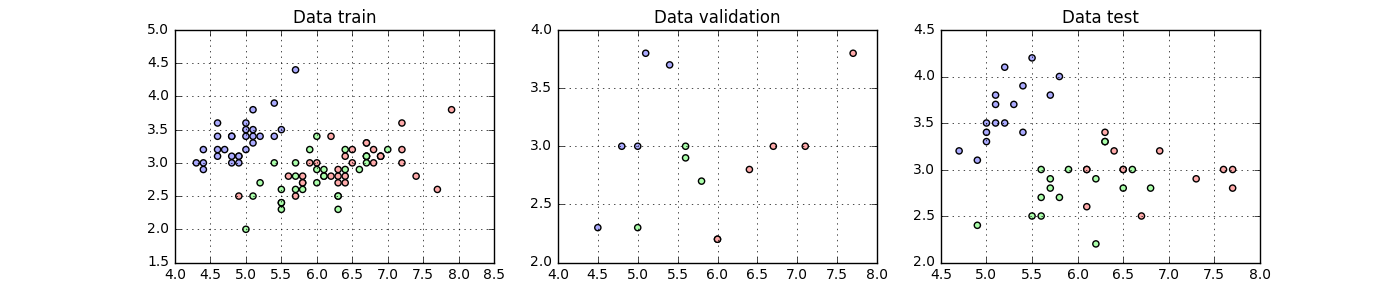
\includegraphics[scale=0.4]{data}
\end{center}

\begin{center}
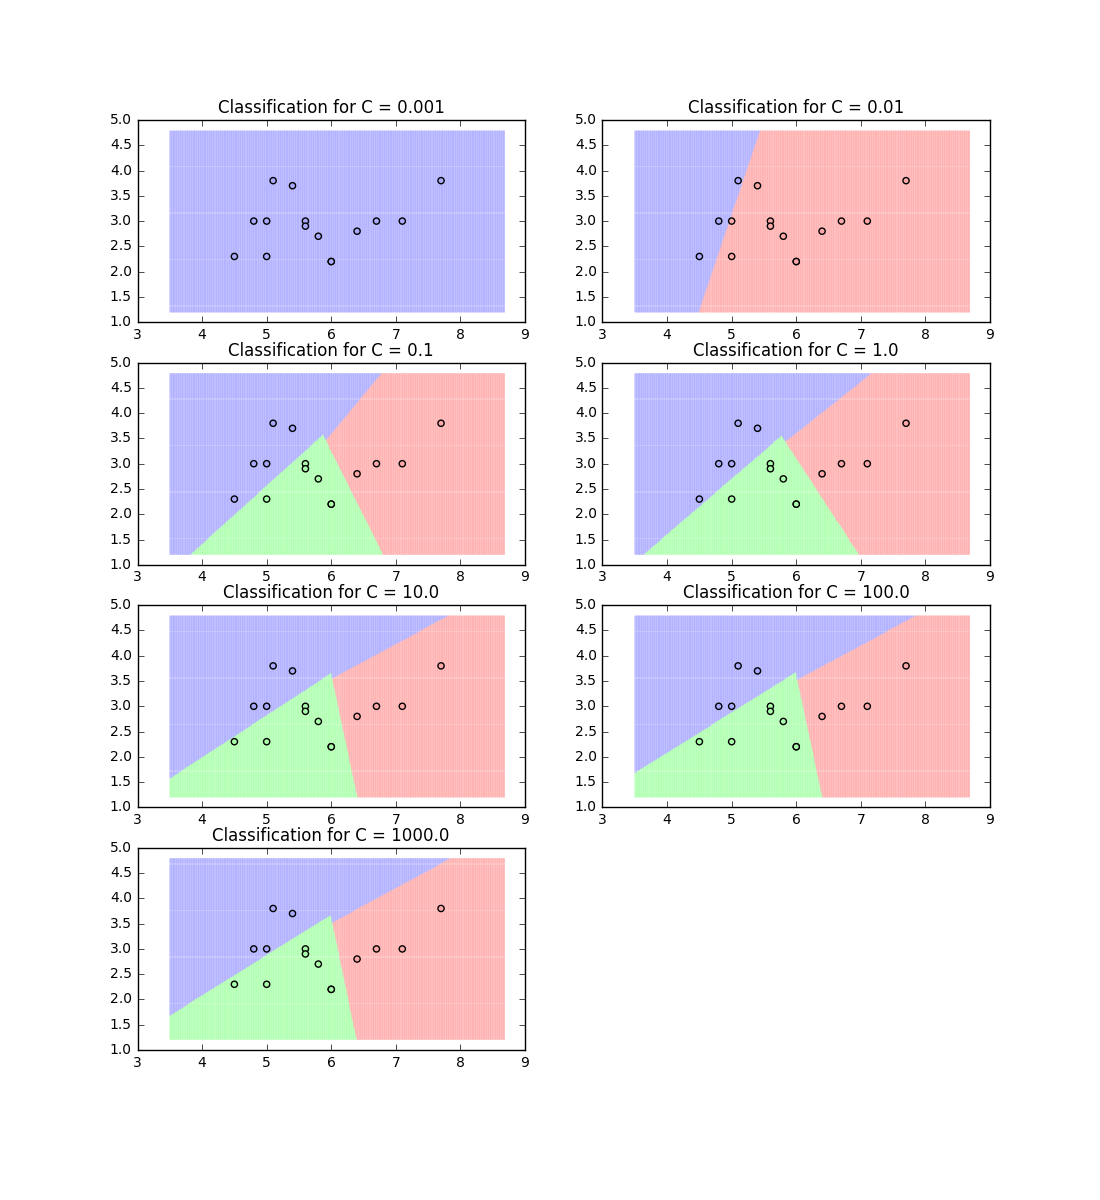
\includegraphics[scale=0.45]{0}
\end{center}

The boundary change accordingly the parameter C that controls the cost of misclassification on the training data. Infact as we can see in the plots , small value of C moves the algorithm to considering a larger margin separator even if this hyperplane could misclassifies the points (soft margin ). Oppositely a large value of C moves to considering smaller margin separetor (hard margin).



\begin{center}
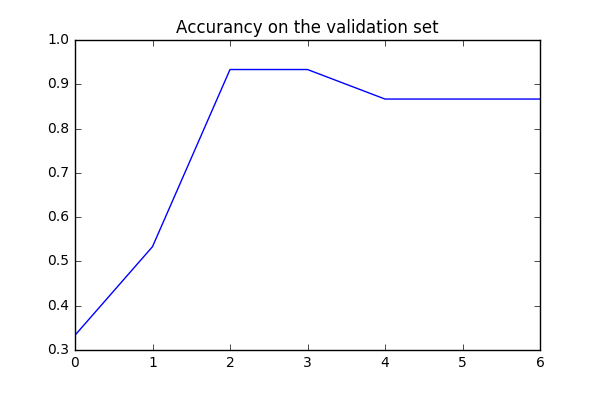
\includegraphics[scale=0.5]{1}
\end{center}

On the validation test we can observe that the best parameter of C wich return the higest accuracy are respectively $C=10^{-1}$ and $C=1$ with both $93.3$\%.



\begin{center}
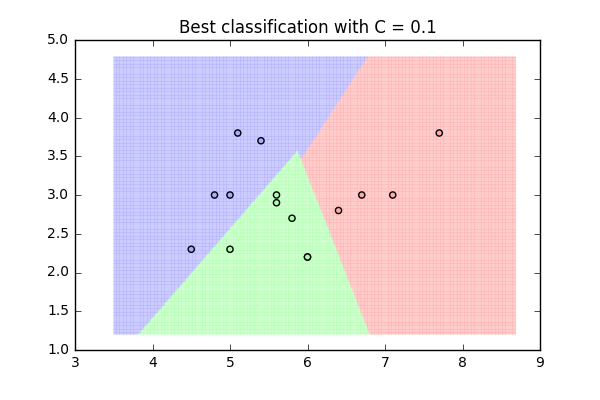
\includegraphics[scale=0.5]{2}
\end{center}

The accuracy obtained with the test data-set in this case is $84.44$\% . One possible consideration is due to the validation data-set have less feature then the test-set , so we have more probability to make a wrong decision. Other is  that for this data-set is unavoidable if commit some error classification and for the case of the validation test we were just lucky with that feature to get an better accuracy.

\newpage

\section{Visualizzation of non linear SVM}
\subsection*{Data}

The same as before , with the same random state in the "train-test-split".

\subsection*{RBF}

\begin{center}
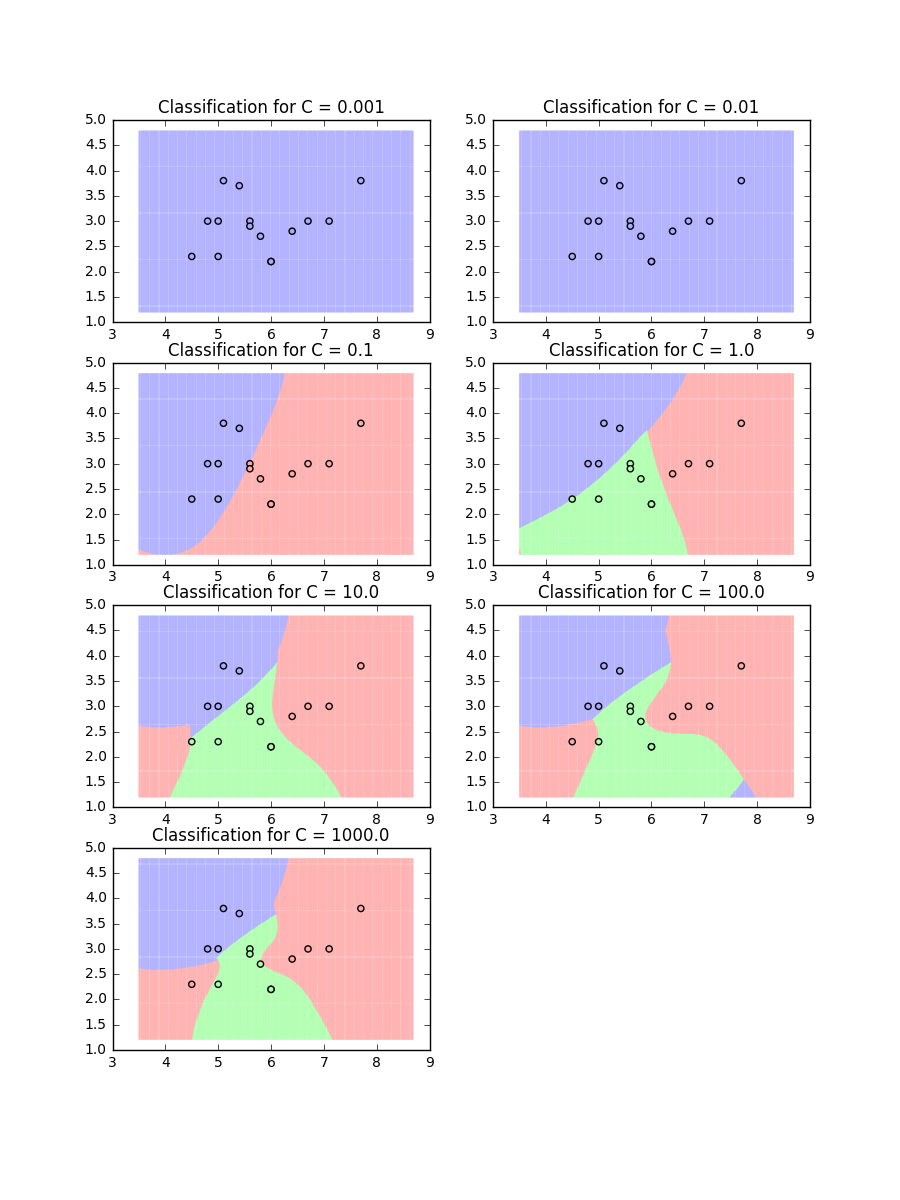
\includegraphics[scale=0.5]{3}
\end{center}

Now as showes from the plot, this kernel allow to curves the margin arround the feature, usually have a more probability to gain some accurancy , especially in the non linear problem. In this case with the validation set we get less accuracy then the linear one . The higher accurancy is riched after $ C = 1 $ with the $86.66$\%.

\begin{center}
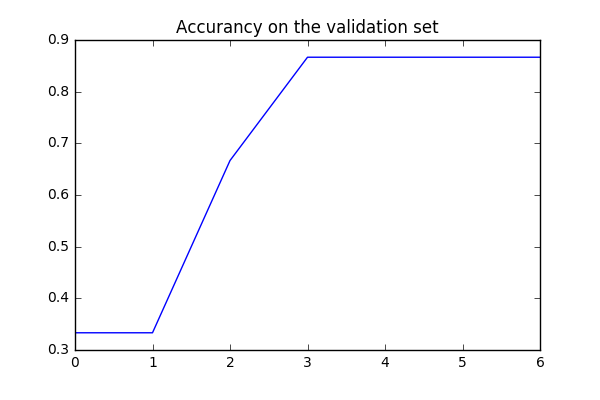
\includegraphics[scale=0.5]{4}
\end{center}

\subsection*{Changing C and Gamma}
Changin C and Gamma with the validation as valutation  : 
\begin{center}
\begin{tabular}{|| r | r | r | r | r | r | r | r ||}
\hline
   Gamma/C    & 0.001    & 0.01     & 0.1      & 1        & 10        & 100        & 1000        \\
   0.01 & 0.333333 & 0.333333 & 0.333333 & 0.666667 &  0.933333 &   0.866667 &    0.866667 \\
   0.1  & 0.333333 & 0.333333 & 0.666667 & 0.933333 &  0.866667 &   0.866667 &    0.866667 \\
   1    & 0.333333 & 0.333333 & 0.666667 & 0.866667 &  0.866667 &   0.866667 &    0.866667 \\
  10    & 0.333333 & 0.333333 & 0.466667 & 0.866667 &  0.733333 &   0.666667 &    0.733333 \\
 100    & 0.333333 & 0.333333 & 0.333333 & 0.533333 &  0.533333 &   0.533333 &    0.533333 \\
\hline
\end{tabular}
\end{center}

\begin{center}
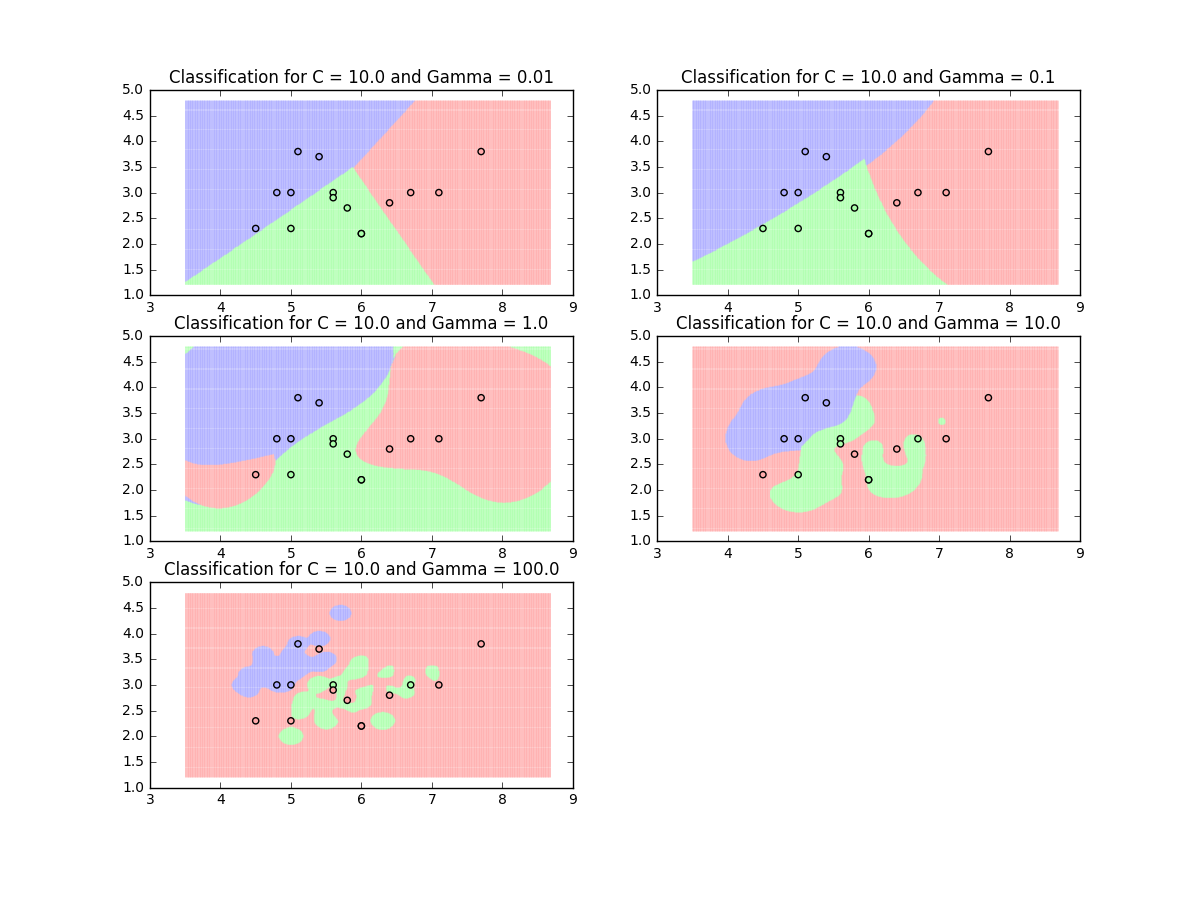
\includegraphics[scale=0.5]{5}
\end{center}

\begin{center}
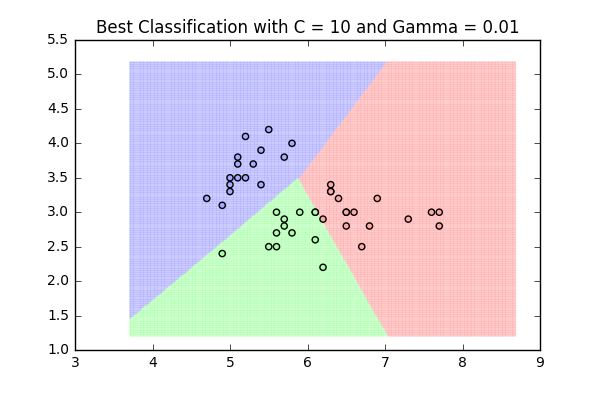
\includegraphics[scale=0.5]{6}
\end{center}

If we consider the better score for the validation set is with $\gamma=0.01$ and $C=100$ we find  an accuracy of $84.44$ \% . But this is not the best score when we classify the test data-set.  Wich in this case result the best one with $\gamma = 1$ and $C =1 $.
\\

\begin{center}
\begin{tabular}{|| r |r |r |r |r |r |r |r ||}
\hline
   Gamma/C    & 0.001    & 0.01     & 0.1      & 1        & 10        & 100        & 1000        \\
   0.01 & 0.288889 & 0.288889 & 0.288889 & 0.644444 &  0.844444 &   0.844444 &    0.844444 \\
   0.1  & 0.288889 & 0.288889 & 0.644444 & 0.844444 &  0.844444 &   0.866667 &    0.844444 \\
   1    & 0.288889 & 0.288889 & 0.666667 & 0.866667 &  0.866667 &   0.844444 &    0.8      \\
  10    & 0.288889 & 0.288889 & 0.511111 & 0.822222 &  0.733333 &   0.733333 &    0.733333 \\
 100    & 0.288889 & 0.288889 & 0.288889 & 0.622222 &  0.622222 &   0.622222 &    0.622222 \\
\hline
\end{tabular}
\end{center}



Score on the test data-set.
\section{K-Fold}
In the basic approach, called k-fold CV, the training set is split into k smaller sets and follow this procedure : 


A model is trained using k-1 of the folds as training data;\\
the resulting model is validated on the remaining part of the data;
\\

\begin{center}
\begin{tabular}{|| r |r |r |r |r | r |r |r ||}
\hline
   Gamma/C    & 0.001    & 0.01     & 0.1      & 1        & 10        & 100        & 1000        \\
   0.01 & 0.428571 & 0.428571 & 0.428571 & 0.714286 &  0.809524 &   0.809524 &    0.857143 \\
   0.1  & 0.428571 & 0.428571 & 0.714286 & 0.809524 &  0.857143 &   0.857143 &    0.857143 \\
   1    & 0.47619  & 0.47619  & 0.857143 & 0.857143 &  0.809524 &   0.809524 &    0.761905 \\
  10    & 0.47619  & 0.47619  & 0.666667 & 0.857143 &  0.714286 &   0.761905 &    0.761905 \\
 100    & 0.380952 & 0.380952 & 0.380952 & 0.666667 &  0.761905 &   0.761905 &    0.761905 \\
\hline
\end{tabular}
\end{center}




Splitting the data using the method of K-fold emprove the accuracy of the most of the test, but not from all.


\end{document}
